\documentclass[10pt,letterpaper]{article}
\usepackage[top=0.85in,left=2.75in,footskip=0.75in]{geometry}

% amsmath and amssymb packages, useful for mathematical formulas and symbols
\usepackage{amsmath,amssymb}

% Use adjustwidth environment to exceed column width (see example table in text)
\usepackage{changepage}

% Use Unicode characters when possible
\usepackage[utf8x]{inputenc}

% textcomp package and marvosym package for additional characters
\usepackage{textcomp,marvosym}

% cite package, to clean up citations in the main text. Do not remove.
\usepackage{cite}

% Use nameref to cite supporting information files (see Supporting Information section for more info)
\usepackage{nameref,hyperref}

% line numbers
\usepackage[right]{lineno}

% ligatures disabled
\usepackage{microtype}
\DisableLigatures[f]{encoding = *, family = * }

% color can be used to apply background shading to table cells only
\usepackage[table]{xcolor}

% array package and thick rules for tables
\usepackage{array}

% enumerate package lets us use letters instead of numbers
\usepackage{enumerate}

% create "+" rule type for thick vertical lines
\newcolumntype{+}{!{\vrule width 2pt}}

% create \thickcline for thick horizontal lines of variable length
\newlength\savedwidth
\newcommand\thickcline[1]{%
  \noalign{\global\savedwidth\arrayrulewidth\global\arrayrulewidth 2pt}%
  \cline{#1}%
  \noalign{\vskip\arrayrulewidth}%
  \noalign{\global\arrayrulewidth\savedwidth}%
}

% \thickhline command for thick horizontal lines that span the table
\newcommand\thickhline{\noalign{\global\savedwidth\arrayrulewidth\global\arrayrulewidth 2pt}%
\hline
\noalign{\global\arrayrulewidth\savedwidth}}

\usepackage{color}

% Remove comment for double spacing
%\usepackage{setspace}
%\doublespacing

% Text layout
\raggedright
\setlength{\parindent}{0.5cm}
\textwidth 5.25in
\textheight 8.75in

% Bold the 'Figure #' in the caption and separate it from the title/caption with a period
% Captions will be left justified
\usepackage[aboveskip=1pt,labelfont=bf,labelsep=period,justification=raggedright,singlelinecheck=off]{caption}
\renewcommand{\figurename}{Fig}

% Use the PLoS provided BiBTeX style
\bibliographystyle{plos2015}

% Remove brackets from numbering in List of References
\makeatletter
\renewcommand{\@biblabel}[1]{\quad#1.}
\makeatother

% Leave date blank
\date{}

% Header and Footer with logo
\usepackage{lastpage,fancyhdr,graphicx}
\usepackage{epstopdf}
\pagestyle{myheadings}
\pagestyle{fancy}
\fancyhf{}
\setlength{\headheight}{27.023pt}
\lhead{
\includegraphics[width=2.0in]{PLOS-submission.eps}}
\rfoot{\thepage/\pageref{LastPage}}
\renewcommand{\footrule}{\hrule height 2pt \vspace{2mm}}
\fancyheadoffset[L]{2.25in}
\fancyfootoffset[L]{2.25in}
\lfoot{\sf PLOS}


%% Define per-paper macros.
\newcommand{\withurl}[2]{{#1}\footnote{\texttt{#2}}}
\newcommand{\rulemajor}[1]{\section{#1}}
\begin{document}
\vspace*{0.2in}

\begin{flushleft}
{\Large
\textbf\newline{Ten Simple Rules for Thinking Like a Programmer}
}
\newline
\\
{Greg~Wilson}\textsuperscript{1,*}
\\
\textbf{1} RStudio, Inc. / greg.wilson@rstudio.com
\\
\bigskip
* Corresponding author.
\end{flushleft}

\section*{Abstract}

FIXME: ABSTRACT

\section*{Author Summary}

FIXME: SUMMARY

\section*{Introduction}

FIXME: INTRODUCTION

The term ``computational thinking'' has been widely used since \cite{Wing2006}
introduced it more than a decade ago.  Unfortunately, it has been used in so
many different ways that no one really knows what it means.

\rulemajor{It's all just data.}

First, and most importantly, it's all just data.  Shopping lists, email,
pictures of far-off galaxies: inside the computer, they're all just ones and
zeroes.  Even programs are just data: in fact, this is the key insight that all
of modern computing is built on.  The source code for a program is just a bunch
of text files, no different from a thesis.  Once that text is compiled or loaded
into memory, it's just bytes too, and pushing those bytes around is no different
from correcting a typo in an address list or changing the color of a pixel in an
image file.  If you understand this—if you understand that programs are just
another kind of data—then every bit of programming you do will be easier.

\rulemajor{Data doesn't mean anything on its own.}

The second idea is a complement to the first: data doesn't mean anything on its
own---it has to be interpreted.  The bits 01100100011000010111100001100001 are
simultaneously the word ``data'', the integer 1,684,108,385, the floating-point
number 1.6635613602263159e+22, a bluish-gray pixel that's slightly transparent,
a medium-loud sound sample with slightly higher volume in the left channel, and
an instruction to copy the content of register 100 to a location in memory
that's 97 bytes past the address currently stored in register 116.

The reason for this is that machines don't understand; they obey.  If you look
at this image, you can't help but see the word ``data'':


\includegraphics{data.png}

A machine doesn't; it doesn't even see four blobs of blue pixels on a gray
background, because it doesn't ``see'' anything.  The computer stores this
image, and a program, as bits in memory.  If those bits happen to correspond to
instructions for the computer's CPU, and if those instructions happen to make up
a program for detecting shapes in images and matching those shapes with letters
in the alphabet, then the computer may very well output ``data'', but \emph{it
  doesn't understand}.  Calling a variable ``temperature'' doesn't mean the
computer will store a temperature in it—it would do exactly the same thing if
the variable was called ``pressure'' or ``frankenstein'' or ``a7''.

\rulemajor{Programming is about creating and composing abstractions.}

This brings us to the third idea: programming is about creating and composing
abstractions.  Our brains can only keep track of a few things at once, so if we
want to understand something, we have to stuff the details into boxes and put
labels on them like ``find the maximum'' or ``patient record''.

One key to making abstraction work is to separate \emph{interface} and
\emph{implementation}.  An interface is what something knows how to do: the
questions it can answer, or the operations it can carry out. Its implementation
is how it does those things: what data it stores, what algorithms it uses, and
so on.  There can be dozens of ways to implement a particular interface; if we
do our work well, we shouldn't have to care about the implementation until
something goes wrong or we need to improve its performance.  ``Spare me the
details'' may be rude in real life, but it's essential in programming.

Another key to making abstraction work is to always choose clarity over
cleverness.  As Brian Kernighan once said, ``{\ldots}debugging is twice as hard
as writing a program in the first place.  So if you are as clever as you can be
when you write it, how will you ever debug it?''  Programs are among the most
complex things human beings have ever created; it may be tempting to use little
tricks here and there to make them smaller or faster, but somebody (maybe you)
is going to have to figure it out again later, and really, nobody likes being
tricked.

\rulemajor{Every redundancy is an abstraction trying to be born.}

FIXME: EXPLAIN (fourth rule).

\rulemajor{Models are for computers, and views are for people.}

Another implication of the abstraction rule is important enough to be our fifth
principle: models are for computers, and views are for people.  A model is a
representation of something that is easy for a computer to operate on; a view is
a way of displaying part or all of that model that human beings can understand.
For example, an HTML document consists of elements with attributes that contain
other elements or blocks of raw text:

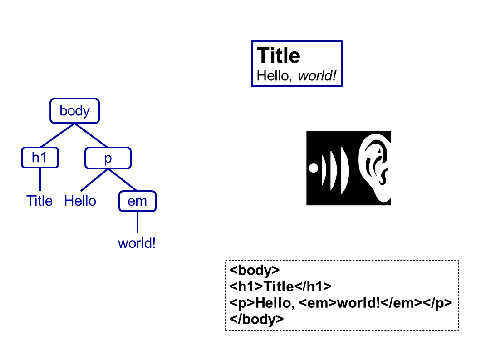
\includegraphics{modelview.png}

That model can be rendered in a browser, turned into speech for someone who is
visually impaired, or displayed as text using angle brackets, quotes, and some
indentation.  None of these \emph{is} the model: they're all views that make the
model's content accessible to human beings in different contexts.  The model
itself isn't just easier for the computer to work with: it's essential, since as
we said before, the computer can't ``see'' the views that we create for human
beings.

Turning one of those views back into a model is hard: parsing the textual
representation of HTML takes thousands of lines of code, and doing OCR or speech
recognition to translate the rendered page or its spoken equivalent can take
millions.  What big idea number four implies, therefore, is that
\emph{structured data is better than unstructured data}.  The tags and
attributes in the textual representation of an HTML page are there because
without it, the computer can't tell whether something is in italics because it's
being emphasized or because it's the title of a book.  To borrow an example from
Jon Udell, a PDF with a cartoon whose caption says, ``The knitting circle meets
on the second Tuesday of every month'' is a lot easier for human beings to
understand than a blob of iCal-formatted text, but the second is much easier for
the computer.

\rulemajor{Paranoia makes us productive.}

We said earlier that we only want to care about how something is implemented
when things go wrong or when we need to improve its performance.  Big idea
number six is about things going wrong, and can be summed up by saying that
\emph{paranoia makes us productive}.  The best way—in fact, the only way—to
improve productivity is to improve quality, and this starts before we write the
first line of code.  ``I want to count all the stars in this photograph'' is easy
to say, but what does it actually \emph{mean}?  What constitutes a star?  When
do you decide that a lumpy blob of pixels is two stars rather than one, or three
instead of two?  Every program embodies decisions about questions like these,
even if you don't realize that there was a question and that you made a choice.
The sooner we worry about this, the less time we'll waste building the wrong
thing.

Of course, we don't stop worrying once we've typed our code in.  We check that
data is formatted properly to protect ourselves against ``garbage in, garbage
out''.  We put checks in our code to make sure that parameters are sensible, data
structures consistent, files aren't empty, and so on.  And we write tests, and
use a build system, to catch errors as soon as possible.  This might feel like
it's slowing us down at first, but study after study has shown that it works.

One of the best ways to apply this principle, by the way, is to automate
everything.  As Alfred North Whitehead said, ``Civilization advances by
extending the number of important operations which we can perform without
thinking about them.''  We don't just write programs because we want to do
things quickly: we write them because we don't want to do some things ever
again.  Version control systems keep track of our work for us; spreadsheets
update graphs and summary statistics whenever a single value changes, and so on.
Every time we automate a task, we reduce the chances of getting it wrong the
next time, and have more time to think about things that machines \emph{can't}
do for us.  And it's not just a one-time saving: if we automate things well,
that extra time is ours over and over again.

\rulemajor{Better algorithms are better than better hardware.}

Big idea number seven is that we can think about how fast the algorithms embodied
in programs are, and that better algorithms are better than better hardware.
One of the greatest mathematical advances of the Twentieth Century was the idea
of \emph{algorithmic complexity}, and its practical implications shape
everything we do with computers, whether we realize it or not.  The basic idea
is that we can estimate how many operations an algorithm will do, or how much
memory it requires, as a function of the size of the problem we're trying to
solve.  It turns out that some algorithms slow down gently as their inputs get
larger, while others slow down so much that even if the whole universe was one
large computer, it couldn't solve any problem big enough to be interesting.
Faster chips help—a lot—but the real key to speed is to focus on what we're
doing, not what we're doing it with.

But algorithms are nothing without data structures to operate on, just as data
structures are pointless without algorithms to manipulate them.  That's why the
two topics are usually taught together: arrays with loops, trees with recursion,
and so on.  Knowing the syntax of this language or the API of that library is
useful, but good programmers know their data structures and algorithms the way a
plumber knows pipes or a musician knows scales.

FIXME: trade space for time for precision (hashing)

\rulemajor{Pass by reference, but appear to pass by value.}

FIXME: RULE (by reference for efficiency and updates, by value because
immutability is easier to understand.

\rulemajor{The street finds its own (mis-)uses for technology (and data).}

The eighth rule is that every decision about what data to collect, who to share
it with, how to analyze it, and how to use the results of those analyses
necessarily and unavoidably furthers someone's interests.

FIXME: CITE Gibson

\rulemajor{The tool shapes the hand.}

Our final rule is something that artisans have known for thousands of years:
\emph{the tool shapes the hand}.  Building software changes how you use
software; making computers do new things changes your understanding of what
computers can do.  That's why any course about computational thinking should ask
you to write software: however frustrating it may sometimes be, it's the only
way to teach you what software can do.

\section*{Conclusion}

An early version of this paper was inspired by Jon Udell's ``Seven Ways to Think
Like the Web'' \cite{Udel2011}.

\bibliography{rules}

\end{document}
